\documentclass[{book}
\usepackage{amsmath}
\begin{document}

\chapter{Phase transitions}
\label{sec:chapter9}

%%%%%%%%%%%%%%%%%%%%%%%%%%%%%%%%%%%%%%%%%%%%%%%%%%%%
\section{Order of phase transition}
We speak of phase transitions when we observe non-analytic behaviour of thermodynamic potentials or their derivatives, while varying thermodynamic variables.

%%%%%%%%%%%%%%%%%%%%
\subsection{First order phase transition}
A first order phase transition is characterized by a discontinuous jump of the expectation value of a thermodynamic potential or its derivative. In \autoref{sec:chapter9} we already encountered an example of this: the discontinuity of the magnetization if the magnetic field changes direction, as sketched in \autoref{fig:chapter8:jump_order_parameter} (recall that $M \sim \phi$ and $B \sim j$). In this example, the thermodynamic potential $\bar{U}$, that needs to be minimized, has two separated local extrema. The absolute minimum changes from one to the other at $B=0$, as illustrated in \autoref{fig:chapter8:modified_effective_potential_different_cases_j}. At $B=0$ both minima have equal $\bar{U}$.

Of course, this is only the special case of a magnetic system. In general, first order phase transitions may occur when varying some other quantity of a system, like temperature or pressure. For example, this is the case for the liquid-gas phase transition. There, the absolute minimum of the corresponding thermodynamic potential changes from liquid to gas phase at $T=\Tc$, as we will work out later in this chapter. It is illustrated in \autoref{fig:chapter9:effective_potential_g1_above_below_critical_temperature}.

%%%%%%%%%%%%%%%%%%%%
\subsection{Second order phase transition}
\label{sec:chapter9:order_of_phase_transition:second_order}
Contrary to a first order phase transition, a second order phase transition is characterized by a continuous behaviour of the expectation value. But susceptibilities or other derivatives diverge. Again, we already encountered an example of this: the magnetization for $j=0$ ($B=0$). In that case, the effective potential was given by
\begin{equation}
  U = \mu^2(T) \rho + \tfrac{1}{2} \lambda \rho^2 \,.
  \label{eq:chapter9:effective_potential_quartic}
\end{equation}
Thereby, $\mu^2(T)$ increases monotonically and $\mu^2(\Tc)=0$. For temperatures $T$ near the critical temperature $\Tc$ it behaves like
\begin{equation}
  \mu^2 = a \, (T-\Tc) + \dotsc \,,
\end{equation}
with some constant $a$. From this the behaviours of $\rho_0$ and $\phi_0$ follow directly:
\begin{alignat}{2}
  \rho_0(T)	&= -\frac{\mu^2(T)}{\lambda}	&&= \frac{a \, (\Tc-T)}{\lambda} \,, \\
  \phi_0(T)	&= \sqrt{2 \rho_0(T)}		&&= c \, \sqrt{\Tc-T} \,,
  \label{eq:chapter9:temperature_dependence_phi0_near_Tc}
\end{alignat}
where $c=\sqrt{\frac{2 a}{\lambda}}$. We already had sketched this behaviour in \autoref{fig:chapter8:phase_diagram_landau_theory}.

In general, one finds $\phi_0$ to behave like a power law near the critical temperature:
\begin{equation}
  \phi_0 \sim (\Tc-T)^\beta \,,
  \label{eq:chapter9:phi0_critical_behaviour}
\end{equation}
with $\beta$ being a so-called critical exponent. In this case $\beta=\frac{1}{2}$ (mean field value).

For our example the derivative of $\phi_0$ with respect to $T$ is given by
\begin{equation}
  \partderiv[\phi_0]{T} \sim \frac{1}{\sqrt{\Tc-T}} \,.
\end{equation}
Indeed, this diverges for $T \rightarrow \Tc$.

Assuming $j\neq0$ again, the effective potential at $\Tc$ is computed as
\begin{equation}
  U = \tfrac{1}{2} \lambda \rho^2 \,,
\end{equation}
and therefore
\begin{equation}
  \bar{U} = \tfrac{1}{8} \lambda \, (\phi_a \phi_a)^2 - j_a \phi_a \,.
\end{equation}
What is the form of $\phi_0(j)$ in this case? To compute it, we take $j_a = j \, \updelta_{a1}$, leading to $\phi_{0,a} = \phi_0 \, \updelta_{a1}$. Then, we find
\begin{equation}
  j = \partderiv[U]{\phi_1} = \frac{\lambda}{2} \phi_0^3 \,,
\end{equation}
and therefore
\begin{equation}
  \phi_0 \sim j^{\nicefrac{1}{3}} \,, \qquad M \sim B^{\nicefrac{1}{3}} \,.
\end{equation}

In general, one finds $M$ to behave like
\begin{equation}
  M \sim B^{\nicefrac{1}{\delta}} \,,
  \label{eq:chapter9:critical_B_dependence_of_magnetization}
\end{equation}
with $\delta$ being another critical exponent. In this case $\delta=3$ (mean field value).

The derivative of $M$ with respect to $B$ is given by
\begin{equation}
  \partderiv[M]{\beta} \sim B^{-\nicefrac{2}{3}} \,,
\end{equation}
which diverges for $B \rightarrow 0$.

The origin of all of this is that the minimum of the thermodynamic potential $U$ splits up into two minima at $T=\Tc$, as shown in Figures \ref{fig:chapter8:effective_potential_symmetric_phase} to \ref{fig:chapter8:effective_potential_phase_transition} (recall that $\mu^2<0$, $\mu^2=0$ and $\mu^2>0$ correspond to $T<\Tc$, $T=\Tc$ and $T>\Tc$, respectively). This is typical for spontaneous symmetry breaking and can occur in other situations, too.

%%%%%%%%%%%%%%%%%%%%
\subsection{Probabilistic interpretation}
The probability to find some value $\phi$ is given by
\begin{equation}
  w(\phi) \sim \exp{-c \bar{U}(\phi)} \,,
\end{equation}
where $c \rightarrow \infty$ in the thermodynamic limit, as $c \sim V$ or $c \sim \N$ for lattice sites. The two non-degenerate local minima of $\bar{U}$ correspond to two local maxima of the probability distribution, as sketched in \autoref{fig:chapter9:probability_distribution_different_temperatures}. Thereby, the relative probability of these two maxima depends on the temperature.

\begin{figure}[t]
  \centering
  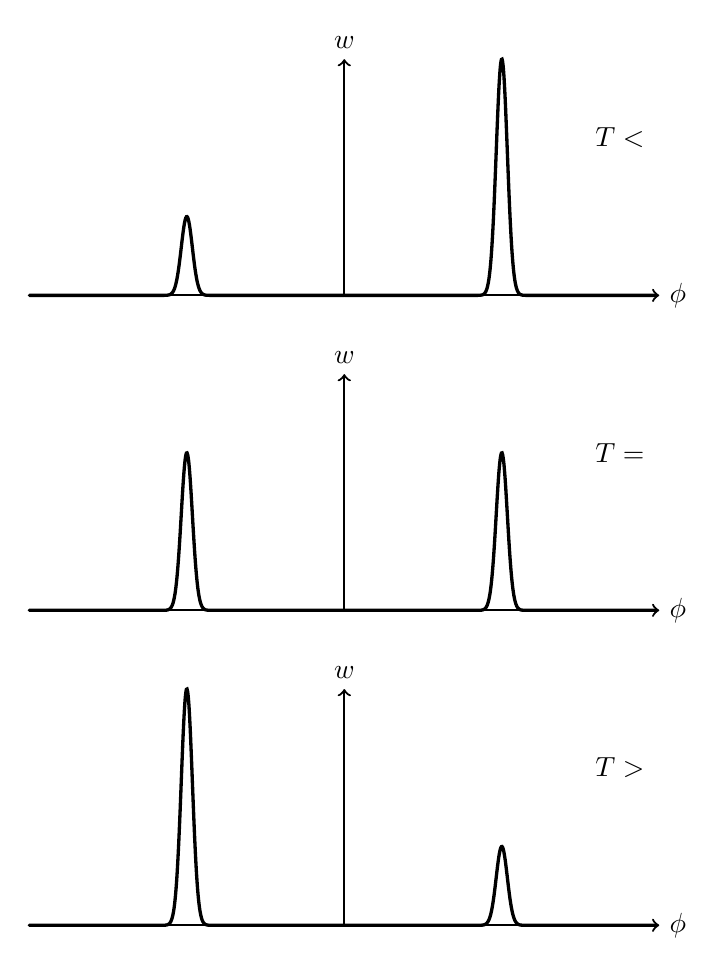
\begin{tikzpicture}[thick]
    \draw[->]
      (0,4) -- (0,7) node[above]{$w$} ;
    \draw[->]
      (-4,4) -- (4,4) node[right]{$\phi$} ;
    \draw[very thick,line cap=round,smooth,domain=-4:0]
      plot[samples=500] (\x, {4+exp(-10^2*(\x+2)^2)}) ;
    \draw[very thick,line cap=round,smooth,domain=0:3.97]
      plot[samples=500] (\x, {4+3*exp(-10^2*(\x-2)^2)}) ;
    \draw
      (3.5,6) node{$T<\Tc$} ;
    %
    \draw[->]
      (0,0) -- (0,3) node[above]{$w$} ;
    \draw[->]
      (-4,0) -- (4,0) node[right]{$\phi$} ;
    \draw[very thick,line cap=round,smooth,domain=-4:0]
      plot[samples=500] (\x, {2*exp(-10^2*(\x+2)^2)}) ;
    \draw[very thick,line cap=round,smooth,domain=0:3.97]
      plot[samples=500] (\x, {2*exp(-10^2*(\x-2)^2)}) ;
    \draw
      (3.5,2) node{$T=\Tc$} ;
    %
    \draw[->]
      (0,-4) -- (0,-1) node[above]{$w$} ;
    \draw[->]
      (-4,-4) -- (4,-4) node[right]{$\phi$} ;
    \draw[very thick,line cap=round,smooth,domain=-4:0]
      plot[samples=500] (\x, {-4+3*exp(-10^2*(\x+2)^2)}) ;
    \draw[very thick,line cap=round,smooth,domain=0:3.97]
      plot[samples=500] (\x, {-4+exp(-10^2*(\x-2)^2)}) ;
    \draw
      (3.5,-2) node{$T>\Tc$} ;
  \end{tikzpicture}
  \caption{Probability distribution for different temperatures}
  \label{fig:chapter9:probability_distribution_different_temperatures}
\end{figure}

\emphpar{“A different state becomes most probable at a first order phase transition.”}

There is a striking phenomenon: The microscopic properties of water molecules are the same for $T<\Tc$ and $T>\Tc$, but a very small change in the average kinetic energy (temperature) produces qualitatively different properties of water and vapor!

%%%%%%%%%%%%%%%%%%%%%%%%%%%%%%%%%%%%%%%%%%%%%%%%%%%%
\section{Liquid-gas phase transition}

%%%%%%%%%%%%%%%%%%%%
\subsection{Effective potential}
The Van der Waals equation of state for real gases is given by
\begin{equation}
  p = \frac{\kB N T}{V - b_0 N} - b_1 \biggl(\frac{N}{V}\biggr)^2 \,,
\end{equation}
with $b_0$, $b_1$ being the so-called virial coefficients. The free energy $F$ is related to the pressure via
\begin{equation}
  \partderiv[F]{V} = -p \,,
\end{equation}
and has the explicit form
\begin{equation}
  F = \kB T N \biggl[\ln{\frac{N}{V - b_0 N}} - 1 - \frac{3}{2} \ln{\frac{m \kB T}{2\pi \hbar^2}}\biggr] - b_1 \frac{N^2}{V} \,.
\end{equation}

In the following we will use the intensive variable $v=\frac{V}{N}=\frac{1}{n}$ (volume per particle). Correspondingly, we define
\begin{equation}
  \tilde{f} = \frac{F}{N} \,,
\end{equation}
such that
\begin{equation}
  \partderiv[\tilde{f}]{v} = -p \,,
\end{equation}
and
\begin{equation}
  \tilde{g}(v,T,p) = \tilde{f}(v,T) + p v \,.
\end{equation}
$\tilde{g}$ plays the role of $\bar{U}$ for magnetic systems, i.\,e. the maximal probability $w(v)$ corresponds to the minimum of $\tilde{g}(v)$:
\begin{equation}
  \partderiv[\tilde{g}]{v}\biggr|_{T,p} = 0.
\end{equation}
In \autoref{tab:chapter9:magnetic_system_vs_real_gas} we have listed the corresponding quantities of magnetic systems and real gases. But note that there is one important difference: there is no $O(N)$-symmetry for the real gas.

\begin{table}[t]
\centering
\begin{tabular}{c c}
\toprule
Magnetic systems	& Real gas \\
\midrule
$\phi$			& $\hphantom{-}v$ \\
$j$			& $-p$ \\
$U$			& $\hphantom{-}\tilde{f}$ \\
$\bar{U}$		& $\hphantom{-}\tilde{g}$ \\
\bottomrule
\end{tabular}
\caption{Magnetic systems vs. real gas}
\label{tab:chapter9:magnetic_system_vs_real_gas}
\end{table}

%%%%%%%%%%%%%%%%%%%%
\subsection{First order transition}
We look for local minima of $\tilde{g}(v)$ for fixed $T$, $p$. Therefore, we split up $\tilde{g}(v)$ into a $v$-dependent and a non-$v$-dependent part:
\begin{equation}
  \tilde{g}(v) = \tilde{g}_0(T) + \tilde{g}_1(v,T,p) \,,
\end{equation}
with ($\kB=\hbar=1$)
\begin{equation}
  \tilde{g}_1 = - T \ln{(v-b_0)} - \frac{b_1}{v} + p v \,,
\end{equation}
leading to
\begin{equation}
  0 = \partderiv[\tilde{g}_1]{v} = - \frac{T}{v-b_0} + \frac{b_1}{v^2} + p \,.
\end{equation}

We find that the equation of state has three solutions for given $T$, $p$ (2 minima, 1 maximum), as sketched in \autoref{fig:chapter9:effective_potential_g1_above_below_critical_temperature}. For $T=\Tc$ both local minima have equal $\tilde{g}_1$. Moreover, there is a jump in density at $T=\Tc$, as shown in \autoref{fig:chapter9:jump_density_liquid_gas_transition}.

\begin{figure}[t]
  \centering
  \subcaptionbox
  {$T<\Tc$
  \label{fig:chapter9:effective_potential_g1_above_below_critical_temperature:below}}[6cm]
  {
    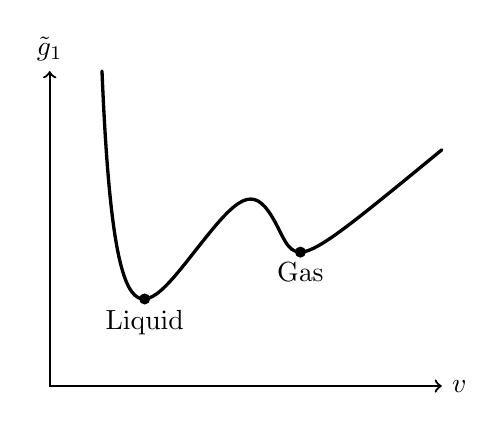
\begin{tikzpicture}[thick,xscale=.83]
      \draw[<->]
        (0,4) node[above]{$\tilde{g}_1$} -- (0,0) -- (6,0) node[right]{$v$} ;
      \draw[very thick,line cap=round]
        (.8,4)
        .. controls (1,0) and (1.5,1) .. (2.5,2)
        node[pos=.56,circle,fill,minimum size=4,inner sep=0]{}
        node[pos=.56,below]{Liquid}
        .. controls (3,2.5) and (3.2,2.5) .. (3.5,2)
        .. controls (3.8,1.5) .. (6,3)
        node[pos=.37,circle,fill,minimum size=4,inner sep=0]{}
        node[pos=.37,below]{Gas} ;
    \end{tikzpicture}
   }
  \hspace{1cm}
  \subcaptionbox
  {$T>\Tc$
  \label{fig:chapter9:effective_potential_g1_above_below_critical_temperature:above}}[6cm]
  {
    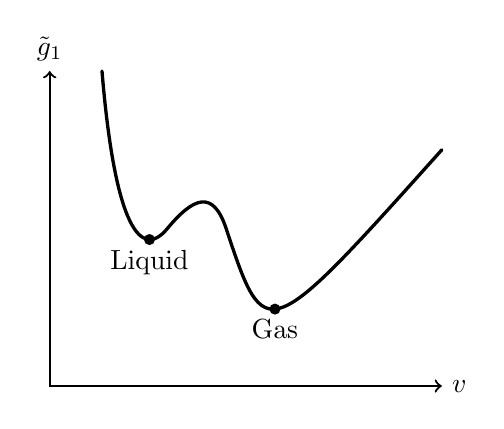
\begin{tikzpicture}[thick,xscale=.83]
      \draw[<->]
        (0,4) node[above]{$\tilde{g}_1$} -- (0,0) -- (6,0) node[right]{$v$} ;
      \draw[very thick,line cap=round]
        (.8,4)
        .. controls (1,2) and (1.4,1.6) .. (1.8,2)
        node[pos=.77,circle,fill,minimum size=4,inner sep=0]{}
        node[pos=.77,below]{Liquid}
        .. controls (2.2,2.4) and (2.5,2.5) .. (2.7,2)
        .. controls (3.3,.5) .. (6,3)
        node[pos=.45,circle,fill,minimum size=4,inner sep=0]{}
        node[pos=.45,below]{Gas} ;
    \end{tikzpicture}
   }
  \caption{Effective potential $\tilde{g}_1$ above and below the critical temperature}
  \label{fig:chapter9:effective_potential_g1_above_below_critical_temperature}
\end{figure}

\begin{figure}[t]
  \centering
  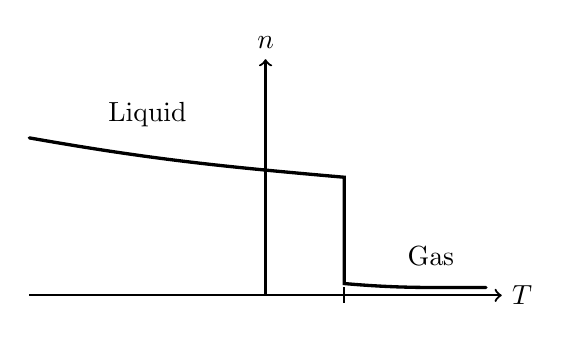
\begin{tikzpicture}[thick]
    \draw[->]
      (0,0) -- (0,3) node[above]{$n$} ;
    \draw[->]
      (-3,0) -- (3,0) node[right]{$T$} ;
    \draw[very thick,line cap=round]
      (-3,2) to[out=-10,in=175] (1,1.5) -- (1,.15) to[out=-5,in=180] (2.8,.1) ;
    \draw
      (1,.1) -- (1,-.1) node[below]{$\Tc$} ;
    \draw
      (-1.5,2.3) node{Liquid}
      (2.1,.5) node{Gas} ;
  \end{tikzpicture}
  \caption{Jump in density during liquid-gas transition}
  \label{fig:chapter9:jump_density_liquid_gas_transition}
\end{figure}

%%%%%%%%%%%%%%%%%%%%
\subsection{Compressibility}
The isothermal compressibility $\kappa_T$ is defined as
\begin{equation}
  \frac{1}{\kappa_T} = - V \partderiv[p]{V}\biggr|_{T,N} \,.
\end{equation}
Note that $\partderiv[p]{V}<0$, as larger pressure corresponds to smaller volume. Therefore $\kappa_T>0$ (if $\kappa_T<0$, this would be an unstable situation).

So, in terms of intensive variables,
\begin{equation}
  \frac{1}{\kappa_T} = -v \partderiv[p]{v} \,,
\end{equation}
and therefore
\begin{equation}
  -\partderiv[p]{v}\biggr|_T = \partderiv{v} \biggl(-\frac{T}{v-b_0} + \frac{b_1}{v^2}\biggr)\biggr|_T \,.
\end{equation}
By comparing this to
\begin{equation}
  \partderiv[\tilde{g}]{v}[2]\biggr|_{T,p} = \partderiv{v} \biggl(-\frac{T}{v-b_0} + \frac{b_1}{v^2}\biggr)\biggr|_T \,,
\end{equation}
we find
\begin{equation}
  \frac{1}{\kappa_T} = v \partderiv[\tilde{g}]{v}[2]\biggr|_{v_0} \,.
\end{equation}
As $\kappa_T>0$, this corresponds to a minimum of $\tilde{g}$. Moreover, we conclude that $\kappa_T v$ corresponds to the susceptibility in magnetic systems.

%%%%%%%%%%%%%%%%%%%%
\subsection{Chemical potential}
The chemical potential is given by
\begin{equation}
  \mu = \tilde{g}(v_0) \,,
\end{equation}
as one can see as follows:
\begin{align}
  \tilde{g}	&= \tilde{f} + p v_0 \\
  		&= \frac{1}{N} (F + p V) \\
  		&= \frac{1}{N} (F - J_{\mathrm{Gibbs}}) \\
  		&= \frac{1}{N} (\mu N) \\
  		&= \mu \,.
\end{align}
Recall that
\begin{equation}
J_{\mathrm{Gibbs}} = F - \mu N = - p V
\end{equation}
and note that $N \tilde{g}$ is the free enthalpy
\begin{equation}
  G(N,T,p) = F + p V \,.
\end{equation}

We are considering chemical reactions where $N$ atoms of a given species can be bound either in molecule A or molecule B. The corresponding variable is the concentration, e.\,g.
\begin{equation}
  c_\B = \frac{\# \text{molecules B}}{\# \text{molecules A} + \# \text{molecules B}} \,.
\end{equation}
It replaces $v$. Then, the probability to find some value $c_\B$ is proportional to $\exp{-\frac{N \tilde{g}(c_\B)}{T}}$.

%%%%%%%%%%%%%%%%%%%%%%%%%%%%%%%%%%%%%%%%%%%%%%%%%%%%
\section{Phase diagram}

%%%%%%%%%%%%%%%%%%%%
\subsection{Vapor pressure curve}
The vapor pressure curve describes the coexistence of fluid and gas at the critical value of $(p,T)$. There are two conditions:
\begin{enumerate}
  \item{$\partderiv[\tilde{g}]{v}=0$, from which we get the equation of state and the solution for the two minima $v_1$, $v_2$ } as a function of $p$,
  \item{$\tilde{g}(v_1)=\tilde{g}(v_2)$, which is equivalent to $\mu_\l=\mu_\g$ (liquid-gas coexistence condition) and from which we get the vapor pressure curve $\pc(T)$.}
\end{enumerate}
So, there is only \emph{one} free parameter (for fixed $N$, $V$), e.\,g. $T$ \emph{or} $p$:
\begin{alignat}{2}
  &\text{given $p$} \quad	&&\rightarrow \quad \Tc \,, \\
  &\text{given $T$} \quad	&&\rightarrow \quad \pc \,.
\end{alignat}

%%%%%%%%%%%%%%%%%%%%
\subsection[\texorpdfstring{$p-T$ diagram}{p-T diagram}]{$\boldsymbol{p-T}$ diagram}
The free enthalpies of the two phases are
\begin{equation}
  G_\l = N_\l \mu_\l(p,T) \,, \qquad G_\g = N_\g \mu_\g(p,T) \,.
\end{equation}
We distinguish the following cases:
\begin{alignat}{2}
  &\mu_\l<\mu_\g: \quad		&&\text{all particles in liquid phase ($N_\l=N$, $N_\g=0$),} \\
  &\mu_\l>\mu_\g: \quad		&&\text{all particles in gas phase ($N_\l=0$, $N_\g=N$),} \\
  &\mu_\l=\mu_\g: \quad	&&\text{transition line ($N_\l, N_\g\neq0$, $N_\l+N_\g=N$).}
\end{alignat}
The transition line is described by $p = \pc(T)$, which we have sketched in \autoref{fig:chapter9:p_T_transition_line_liquid_gas}. So, coexistence in equilibrium is possible. Note that this is a universal curve, as it is independent of $N_\l$, $N_\g$.

\begin{figure}[t]
  \centering
  \begin{tikzpicture}[thick]
    \draw[<->]
      (0,4) node[above]{$p$} -- (0,0) -- (6,0) node[right]{$T$} ;
    \draw[very thick,line cap=round]
      (0,.5) to[out=10,in=240] (5,3.5) node[right]{$\mu_\l=\mu_\g$} ;
    \draw
      (2,3) node{Liquid}
      (2,2.5) node{$\mu_\l<\mu_\g$}
      (4.5,1) node{Gas}
      (4.5,.5) node{$\mu_\l>\mu_\g$} ;
  \end{tikzpicture}
  \caption{$p-T$ transition line between liquid and gas phase}
  \label{fig:chapter9:p_T_transition_line_liquid_gas}
\end{figure}

%%%%%%%%%%%%%%%%%%%%
\subsection{Clausius-Clapeyron relation}
We can set up a differential equation for the transition line by combining the coexistence conditions of two infinitesimally distant points on the transition line (changing the index notation from l,g to 1,2):
\begin{align}
  \mu_1(T,p)			&= \mu_2(T,p) \,, \\
  \mu_1(T+\d T,p+\d p)	&= \mu_2(T+\d T,p+\d p) \,,
\end{align}
to arrive at
\begin{equation}
  \d\mu_1 = \d\mu_2 \,,
  \label{eq:chapter9:differential_coexistence}
\end{equation}
with
\begin{equation}
  \d\mu_i = \underbrace{\partderiv[\mu_i]{T}}_{-\tfrac{S}{N}} \d T + \underbrace{\partderiv[\mu_i]{p}}_{\tfrac{V}{N}} \d p \,.
\end{equation}
The latter is the so-called Duhem-Gibbs relation:
\begin{equation}
  \d\mu = \frac{V}{N} \d p - \underbrace{\frac{S}{N}}_{\tilde{s}} \d T \,.
\end{equation}
When expressing it in terms of intensive quantities and combining it with \eqref{eq:chapter9:differential_coexistence} we arrive at
\begin{equation}
  v_1 \d p - \tilde{s}_1 \d T = v_2 \d p - \tilde{s}_2 \d T \,,
\end{equation}
which we can rewrite as
\begin{equation}
  \underbrace{(\tilde{s}_2 - \tilde{s}_1)}_{\Delta\tilde{s}} \d T = \underbrace{(v_2 - v_1)}_{\Delta v} \d\pc \,,
\end{equation}
to find the Clausius-Clapeyron equation:
\begin{equation}
  \frac{\d\pc}{\d T} = \frac{\Delta\tilde{s}}{\Delta v} \,.
\end{equation}
It tells us that the slope of $\pc(T)$ is given by the ratio of entropy difference and volume difference.

%%%%%%%%%%%%%%%%%%%%
\subsection{Latent heat}
There is a jump in entropy at the phase transition. So, heat has to be absorbed or released (the phase transition can also be adiabatic if the change in $T$ is slow). It is called “latent heat” and is given by
\begin{equation}
  L_{12} = T \Delta S = T (S_2 - S_1) \,.
\end{equation}
Combining it with the Clausius-Clapeyron equation gives us
\begin{equation}
  \boxed{
    L_{12} = \totderiv[T]{\pc} T \, \Delta V \,.
  }
\end{equation}
The latent heat is necessary to separate the water molecules during the transition from the liquid to the gas phase or to break up the crystal structure during the transition from the ice (solid) to the liquid phase, respectively.

%%%%%%%%%%%%%%%%%%%%
\subsection{Superheating, supercooling}
Let us introduce the following time scales:
\begin{customlist}{$t_\A$:}
  \item[$t_\A$:]{typical time scale of establishing the equilibrium in the liquid (relaxation time),}
  \item[$t_\B$:]{typical time scale of establishing the equilibrium in the gas,}
  \item[$t_\T$:]{time scale of the liquid-gas transition (forming of droplets\,/\,bubbles).}
\end{customlist}
For $T<\Tc$ the probability to be in the gas phase is much smaller than the probability to be in the liquid phase:
\begin{equation}
  w_\B \ll w_\A \,,
\end{equation}
as sketched in \autoref{fig:chapter9:probability_distributions_liquid_gas}. But for the states in between these two phases it is even smaller:
\begin{equation}
  w(v) \ll w_\B \quad \text{for $v_\A < v < v_\B$} \,.
\end{equation}
Therefore, small fluctuations near B, e.\,g. at $x$, tend to return to B (stability of B regarding small fluctuations). An equivalent explanation would be to say that B is a local minimum of $G$, even if $T<\Tc$, as illustrated in \autoref{fig:chapter9:free_enthalpy_liquid_phase}.

\begin{figure}[t]
  \centering
  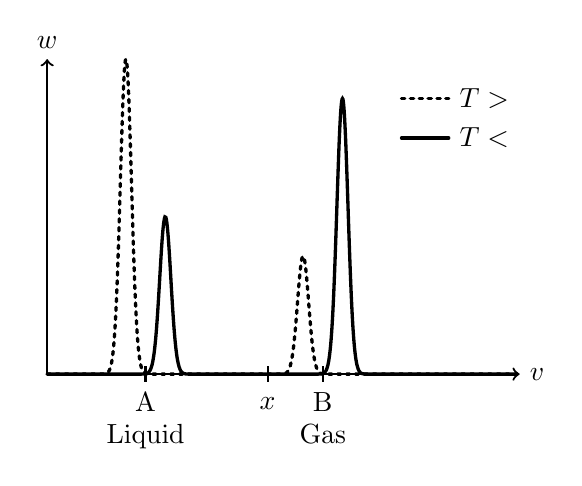
\begin{tikzpicture}[thick]
    \draw[<->]
      (0,4) node[above]{$w$} -- (0,0) -- (6,0) node[right]{$v$} ;
    \draw[very thick,line cap=round,smooth,domain=0:5.97]
      plot[samples=500] (\x, {2*exp(-10^2*(\x-1.5)^2)+3.5*exp(-10^2*(\x-3.75)^2)}) ;
    \draw[very thick,dotted,line cap=round,smooth,domain=0:5.97]
      plot[samples=500] (\x, {4*exp(-10^2*(\x-1)^2)+1.5*exp(-10^2*(\x-3.25)^2)}) ;
    \draw[very thick,dotted,line cap=round]
      (4.5,3.5) -- (5.1,3.5) node[right]{$T>\Tc$} ;
    \draw[very thick,line cap=round]
      (4.5,3) -- (5.1,3) node[right]{$T<\Tc$} ;
    \draw
      (1.25,.1) --(1.25,-.1) node[below]{A}
      (1.25,-.5) node[below]{Liquid}
      (3.5,.1) -- (3.5,-.1) node[below]{B}
      (3.5,-.5) node[below]{\vphantom{Liquid}Gas}
      (2.8,.1) -- (2.8,-.1) node[below=2]{$x$} ;
  \end{tikzpicture}
  \caption{Probability distributions for liquid and gas phase}
  \label{fig:chapter9:probability_distributions_liquid_gas}
\end{figure}

\begin{figure}[t]
  \centering
  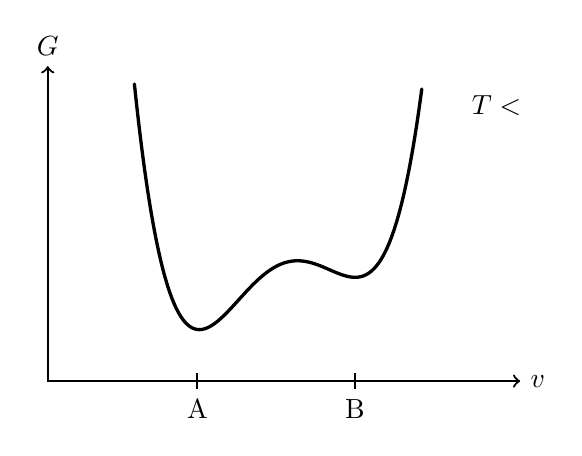
\begin{tikzpicture}[thick]
    \draw[<->]
      (0,4) node[above]{$G$} -- (0,0) -- (6,0) node[right]{$v$} ;
    \draw[very thick,line cap=round,domain=1.1:4.75]
      plot[samples=200] (\x, {1.5-(\x-3)^2+((\x-3)^4)/2+(\x-3)/3}) ;
    \draw
      (5.7,3.5) node{$T<\Tc$}
      (1.9,.1) -- (1.9,-.1) node[below]{A}
      (3.9,.1) -- (3.9,-.1) node[below]{B} ;
  \end{tikzpicture}
  \caption{Free enthalpy in liquid phase}
  \label{fig:chapter9:free_enthalpy_liquid_phase}
\end{figure}

The typical time scale of a fluctuation returning to B is given by $t_\B$, which is usually much shorter than $t_\T$ (overcoming a barrier; similar to tunneling in QM: exponentially suppressed probabilities). Let us now consider an experimental time scale $t_\E$ in between these:
\begin{equation}
  t_\B \ll t_\E \ll t_\T \,.
\end{equation}
In this case, the system has not enough time for the transition $\mathrm{B} \rightarrow \mathrm{A}$, but instead stays in the “local” equilibrium B even beyond the critical point. This phenomenon is called supercooling (one speaks of superheating if during the transition $\mathrm{A} \rightarrow \mathrm{B}$ the systems stays in A beyond the critical point). Eventually, the local instability will become extremal when B becomes a saddle point and finally a maximum. In practice one can observe the coexistence of water and vapor not only at $\Tc$.

For magnets the same effect appears in the form of hysteresis. Indeed, this is a characteristic effect for \emph{first} order transitions in general.
\end{document}